%% 
%% Copyright 2007, 2008, 2009 Elsevier Ltd
%% 
%% This file is part of the 'Elsarticle Bundle'.
%% ---------------------------------------------
%% 
%% It may be distributed under the conditions of the LaTeX Project Public
%% License, either version 1.2 of this license or (at your option) any
%% later version.  The latest version of this license is in
%%    http://www.latex-project.org/lppl.txt
%% and version 1.2 or later is part of all distributions of LaTeX
%% version 1999/12/01 or later.
%% 
%% The list of all files belonging to the 'Elsarticle Bundle' is
%% given in the file `manifest.txt'.
%% 

%% Template article for Elsevier's document class `elsarticle'
%% with numbered style bibliographic references
%% SP 2008/03/01
%%
%% 
%%
%% $Id: elsarticle.cls,v 1.20 2008-10-13 04:24:12 cvr Exp $
%%
%%
\documentclass[preprint,12pt]{elsarticle}

%% Use the option review to obtain double line spacing
%% \documentclass[preprint,review,12pt]{elsarticle}

%% Use the options 1p,twocolumn; 3p; 3p,twocolumn; 5p; or 5p,twocolumn
%% for a journal layout:
%% \documentclass[final,1p,times]{elsarticle}
%% \documentclass[final,1p,times,twocolumn]{elsarticle}
%% \documentclass[final,3p,times]{elsarticle}
%% \documentclass[final,3p,times,twocolumn]{elsarticle}
%% \documentclass[final,5p,times]{elsarticle}
%% \documentclass[final,5p,times,twocolumn]{elsarticle}

%% if you use PostScript figures in your article
%% use the graphics package for simple commands
%% \usepackage{graphics}
%% or use the graphicx package for more complicated commands
%% \usepackage{graphicx}
%% or use the epsfig package if you prefer to use the old commands
%% \usepackage{epsfig}

%% The amssymb package provides various useful mathematical symbols
\usepackage{amssymb}
%% The amsthm package provides extended theorem environments
%% \usepackage{amsthm}


% the following package is optional:
\usepackage{latexsym} 
\usepackage{amsmath}

\usepackage{subfigure}
\usepackage{xspace}
\usepackage{url}

% Load pfg package for drawing transition systems
\usepackage{tikz,pgf}
\usetikzlibrary{arrows,automata,trees,plotmarks,calc}


\usepackage{algorithm}
\usepackage{algorithmic}
%\usepackage[ruled,vlined]{algorithm2e}




%% The lineno packages adds line numbers. Start line numbering with
%% \begin{linenumbers}, end it with \end{linenumbers}. Or switch it on
%% for the whole article with \linenumbers after \end{frontmatter}.
%% \usepackage{lineno}

%% natbib.sty is loaded by default. However, natbib options can be
%% provided with \biboptions{...} command. Following options are
%% valid:

%%   round  -  round parentheses are used (default)
%%   square -  square brackets are used   [option]
%%   curly  -  curly braces are used      {option}
%%   angle  -  angle brackets are used    <option>
%%   semicolon  -  multiple citations separated by semi-colon 
%%   colon  - same as semicolon, an earlier confusion
%%   comma  -  separated by comma
%%   numbers-  selects numerical citations
%%   super  -  numerical citations as superscripts
%%   sort   -  sorts multiple citations according to order in ref. list
%%   sort&compress   -  like sort, but also compresses numerical citations
%%   compress - compresses without sorting
%%
%% \biboptions{comma,round}

% \biboptions{}


\journal{Nuclear Physics B}







%%%%%%%%%%%%%%%%%%%%%%%%%%%%%%%%%%%%%%%%%%%%%%%%%%%%%%%%%%%%%%%%%%%%%%%%
%%%%% START OF MACROS
%%%%%%%%%%%%%%%%%%%%%%%%%%%%%%%%%%%%%%%%%%%%%%%%%%%%%%%%%%%%%%%%%%%%%%%%
%%%%%%%%%%%%%%%%%%%%%%%%%%%%%%%%%%%%%%%%%%%%%%%%%%%%
% PERSONAL LaTex MACROS 
%	SEBASTAN SARDINA -- ssardina@cs.rmit.edu.au
%%%%%%%%%%%%%%%%%%%%%%%%%%%%%%%%%%%%%%%%%%%%%%%%%%%%



%%%%%%%%%%%%%%%%%%%%%%%%%%%%%%%%%%%%%%%%%%%%%%%%%%%%
% Font modes & definitions
%%%%%%%%%%%%%%%%%%%%%%%%%%%%%%%%%%%%%%%%%%%%%%%%%%%%

% conditional math environment
% \gdef\Math#1{\ifmmode #1 \else \mbox{$#1$}\fi}
\newcommand{\Math}[1]{\ensuremath{#1}}



\newcommand{\modesf}[1]{{\Math{\mathsf{#1}}}}
\newcommand{\modecal}[1]{{\Math{\mathcal{#1}}}}
\newcommand{\modeit}[1]{{\Math{\mathit{#1}}}}


\newcommand{\textmath}[1]{{\mbox{\textit{#1}}}}


%%%%%%%%%%%%%%%%%%%%%%%%%%%%%%%%%%%%%%%%%%%%%%%%%%%%
% Proper names
%%%%%%%%%%%%%%%%%%%%%%%%%%%%%%%%%%%%%%%%%%%%%%%%%%%%
\newcommand{\propername}[1]{\mbox{\small \textsf{#1}}}

\newcommand{\Golog}{\propername{Golog}}
\newcommand{\GologSpeak}{\propername{GologSpeak}}
\newcommand{\DGolog}{\propername{DGolog}}
\newcommand{\sGolog}{\propername{sGolog}}
\newcommand{\ConGolog}{\propername{ConGolog}}
\newcommand{\IndiGolog}{\propername{IndiGolog}}
\newcommand{\LeGolog}{\propername{LeGolog}}
\newcommand{\DTGolog}{\propername{DTGolog}}
\newcommand{\Prolog}{\propername{Prolog}}
\newcommand{\AgentSpeak}{\propername{AgentSpeak}}
\newcommand{\JASON}{\propername{Jason}}
\newcommand{\CANMINUS}{\propername{\CAN$^{\A}$}}
\newcommand{\CANMINUST}{\propernametiny{Can$^{\cal C}$}}
\newcommand{\CAN}{\propername{CAN}}
\newcommand{\CANT}{\propernametiny{Can}}
\newcommand{\CANPLAN}{\propername{CANPlan}}
\newcommand{\CANPLANT}{\propernametiny{CanPlan}}
\newcommand{\CANPLANII}{\propername{CanPlan2}}
\newcommand{\CANPLANOR}{\propername{Can(Plan)}}
\newcommand{\CANGOAL}{\propername{CanGoal}}
\newcommand{\JACK}{\propername{JACK}}
\newcommand{\weka}{\propername{weka}}
\newcommand{\JACKTM}{\propername{Jack\texttrademark}}
\newcommand{\JAM}{\propername{JAM}}
\newcommand{\DAPL}{\propername{2APL}}
\newcommand{\GOAL}{\propername{GOAL}}
\newcommand{\PRS}{\propername{PRS}}
\newcommand{\SPARK}{\propername{SPARK}}
\newcommand{\RAP}{\propername{Rap}}
\newcommand{\dMARS}{\propername{dMARS}}
\newcommand{\TAPL}{\propername{3APL}}
\newcommand{\GOALBDI}{\propername{GOAL}}
\newcommand{\JSHOP}{\propername{JSHOP}}
\newcommand{\JSHOPII}{\propername{JSHOP2}}
\newcommand{\ASHOP}{\propername{A-SHOP}}
\newcommand{\SHOP}{\propername{SHOP}}
\newcommand{\SHOPII}{\propername{SHOP2}}
\newcommand{\ACT}{\propername{ACT}}
\newcommand{\SIPEII}{\propername{SIPE-2}}
\newcommand{\OPLANII}{\propername{O-PLAN2}}
\newcommand{\Retsina}{\propername{Retsina}}
\newcommand{\IPEM}{\propername{IPEM}}
\newcommand{\SAGE}{\propername{Sage}}
\newcommand{\DECAF}{\propername{Decaf}}
\newcommand{\PROPICE}{\propername{Propice-Plan}}
\newcommand{\CYPRESS}{\propername{Cypress}}
\newcommand{\CPEF}{\propername{CPEF}}
\newcommand{\JADEX}{\propername{JADEX}}
\newcommand{\IMPACT}{\propername{IMPACT}}
\newcommand{\PDT}{\propername{PDT}}


%%%%%%%%%%%%%%%%%%%%%%%%%%%%%%%%%%%%%%%%%%%%%%%%%%%%
% Calligraphic letters - Taken from Giuseppe De Giacomo 2006
%%%%%%%%%%%%%%%%%%%%%%%%%%%%%%%%%%%%%%%%%%%%%%%%%%%%
\newcommand{\A}{\modecal{A}} \newcommand{\B}{\modecal{B}}
\newcommand{\C}{\modecal{C}} \newcommand{\D}{\modecal{D}}
\newcommand{\E}{\modecal{E}} \newcommand{\F}{\modecal{F}}
\newcommand{\G}{\modecal{G}} \renewcommand{\H}{\modecal{H}}
\newcommand{\I}{\modecal{I}} \newcommand{\J}{\modecal{J}}
\newcommand{\K}{\modecal{K}} \renewcommand{\L}{\modecal{L}}
\newcommand{\M}{\modecal{M}} \newcommand{\N}{\modecal{N}}
\renewcommand{\O}{\modecal{O}} \renewcommand{\P}{\modecal{P}}
\renewcommand{\S}{\modecal{S}} \newcommand{\T}{\modecal{T}}
\newcommand{\U}{\modecal{U}} \newcommand{\V}{\modecal{V}}
\newcommand{\W}{\modecal{W}} \newcommand{\X}{\modecal{X}}
\newcommand{\Y}{\modecal{Y}} \newcommand{\Z}{\modecal{Z}}
\newcommand{\R}{\modecal{R}} 



%%%%%%%%%%%%%%%%%%%%%%%%%%%%%%%%%%%%%%%%%%%%%%%%%%%%
% Situation Calculus macros
%%%%%%%%%%%%%%%%%%%%%%%%%%%%%%%%%%%%%%%%%%%%%%%%%%%%

% Sitcalc Golog/ConGolog/IndiGolog programs
\newcommand{\mif}{\mbox{\bf if}}
\newcommand{\mwhile}{\mbox{\bf while}}
\newcommand{\mreturn}{\mbox{\bf return}}
\newcommand{\mthen}{\mbox{\bf then}}
\newcommand{\melse}{\mbox{\bf else}}
\newcommand{\mdo}{\mbox{\bf do}}
\newcommand{\mnoOp}{\mbox{\bf $noOp$}}
\newcommand{\mproc}{\mbox{\bf proc}}
\newcommand{\mend}{\mbox{\bf end}}
\newcommand{\mendproc}{\mbox{\bf endProc}}
\newcommand{\mendif}{\mbox{\bf endIf}}
\newcommand{\mendwhile}{\mbox{\bf endWhile}}
\newcommand{\mendfor}{\mbox{\bf endFor}}
\newcommand{\mfor}{\mbox{\bf for}}
\def\prparallel{\mathrel{\rangle\!\rangle}}
\def\supparallel{\mathord{|\!|}}
\newcommand{\conc}{\mbox{$\parallel$}}
\newcommand{\pconc}{\mbox{$\prparallel$}}
\newcommand{\search}{\mbox{$\Sigma$}}
\newcommand{\searchO}{\mbox{$\Sigma_o$}}
\newcommand{\searchOM}{\mbox{$\Sigma_o^M$}}
\newcommand{\searchCR}{\mbox{$\Sigma_{cr}$}}
\newcommand{\searchR}{\mbox{$\Sigma_{r}$}}
\newcommand{\searchM}{\mbox{$\Sigma^M$}}
\newcommand{\searchC}{\mbox{$\Sigma_c$}}
\newcommand{\searchCM}{\mbox{$\searchC^M$}}
\newcommand{\searchCB}{\mbox{$\Sigma_{cb}$}}
\newcommand{\searchD}{\mbox{$\Delta$}}
\newcommand{\searchE}{\mbox{$\Delta_e$}}
\newcommand{\searchEM}{\mbox{$\Delta_e^M$}}
\newcommand{\searchL}{\mbox{$\Delta_l$}}
\newcommand{\searchER}{\mbox{$\Delta_r$}}
\newcommand{\searchERM}{\mbox{$\Delta_r^M$}}
\newcommand{\mnt}{\mbox{$mnt$}}


%%% Knowledge in sitcalc
\newcommand{\Know}{\mbox{\bf Know}}
\newcommand{\KWhether}{\mbox{\bf KWhether}}
\newcommand{\Kref}{\mbox{\bf KRef}}
\newcommand{\nows}{{\hbox{\small\sf now}}}
\newcommand{\now}{{\mbox{\sf now}}}


% IndiGolog macros
\newcommand{\Sensed}{\textmath{Sensed}}
\newcommand{\hend}{\textmath{end}}
\newcommand{\Trans}{\textmath{Trans}}
\newcommand{\Final}{\textmath{Final}}
\newcommand{\Poss}{\textmath{Poss}}
\newcommand{\Transobs}{\textmath{TransObs}}


%%%%%%%%%%%%%%%%%%%%%%%%%%%%%%%%%%%%%%%%%%%%%%%%%%%%
% CAN notation for BDI Agents
%%%%%%%%%%%%%%%%%%%%%%%%%%%%%%%%%%%%%%%%%%%%%%%%%%%%
\newcommand{\Goal}{\modesf{Goal}}
\newcommand{\GoalS}{\modesf{G}}
\newcommand{\SGoal}{\modesf{SGoal}}
\newcommand{\SGoalS}{\modesf{SG}}
\newcommand{\goal}[3]{{\sf Goal}(#1,#3,#2)}
\newcommand{\goalp}[3]{{\sf Goal}_{P}(#1,#3,#2)}
\newcommand{\goalsfp}{\goal{s}{f}{P}}
\newcommand{\goalsfpp}{\goalp{s}{f}{P}}
\newcommand{\goalt}[2]{{\sf Goal}(#1,#2)}
\newcommand{\goalsf}{\goal{s}{f}}

\newcommand{\Plan}{\modesf{Plan}}
\newcommand{\PlanP}{\modesf{P}}
\newcommand{\PlanArg}[1]{\Plan(#1)}

\newcommand{\pnil}{\mbox{\textit{nil}}}
\newcommand{\ptrue}{\mbox{\textit{true}}}
\newcommand{\pfalse}{\mbox{\textit{false}}}
\newcommand{\pfail}{\mbox{\textit{fail}}}

\newcommand{\pguardaltl}[1]{\mbox{$\altl #1 \altr$}} % guarded alternatives
\newcommand{\altl}{\llparenthesis}
\newcommand{\altr}{\rrparenthesis}

%% Macro for BDI plan rules:  \plane{a:b<-c} \plans{a<-c}
\newcommand\plane[1]{\planeaux!#1!}
\def\planeaux!#1:#2<-#3!{\Math{#1 \mbox{\rm:} #2\; \leftarrow #3}}
\newcommand\plans[1]{\planeaux!#1!}
\def\planeaux!#1<-#2!{\Math{#1 \leftarrow #2}}




%%%%%%%%%%%%%%%%%%%%%%%%%%%%%%%%%%%%%%%%%%%%%%%%%%%%
% START - Operational semantics
%%%%%%%%%%%%%%%%%%%%%%%%%%%%%%%%%%%%%%%%%%%%%%%%%%%%
% Labels
\newcommand{\bdi}{bdi}
\newcommand{\htn}{plan}
\newcommand{\transitionlabel}[1]{\modesf{{#1}}}

% Meta-transition
\newcommand{\mtransition}{\Longrightarrow} % meta transition
\newcommand{\mtransitionstar}{\overset{*}{\mtransition}} % trans meta closure
\newcommand{\mtransitiontype}[1]{\overset{\transitionlabel{#1}}{\mtransition}}
\newcommand{\mtransitionstartype}[1]{\overset{*}{\mtransitiontype{#1}}}

% Transition
\newcommand{\transition}{\longrightarrow} 	% regular transition

\newcommand{\transitionstar}{\overset{*}{\transition}} % trans closure
\newcommand{\transitionst}{\overset{*}{\transition}} %trans closure
\newcommand{\transitionanot}[1]{\transition_{#1}} 	% regular transition
\newcommand{\transitionbdistarint}
	{\overset{\transitionlabel{\bdi}_{*}}{\transition_i}}

\newcommand{\transitiontype}[1]{\overset{\transitionlabel{#1}}{\transition}}
\newcommand{\transitionbdi}{\overset{\transitionlabel{\bdi}}{\transition}}
\newcommand{\transitionhtn}{\overset{\transitionlabel{\htn}}{\transition}}
\newcommand{\transitionhtnstar}
	{\overset{\transitionlabel{\htn}_{*}}{\transition}}
\newcommand{\transitionbdistar}
{\overset{\transitionlabel{\bdi}_{*}}{\transition}}

\newcommand{\transitionhtnk}[1]
{\overset{\transitionlabel{\htn}_{#1}}{\transition}}
\newcommand{\transitionbdik}[1]
{\overset{\transitionlabel{\bdi}_{#1}}{\transition}}



%%%%%%%%%%%%%%%%%%%%%%%%%%%%%%%%%%%%%%%%%%%%%%%%%%%%
% Several notations
%%%%%%%%%%%%%%%%%%%%%%%%%%%%%%%%%%%%%%%%%%%%%%%%%%%%

%%%%%%%%%%%%%%%%%%%%%%%%%% Delimiters
\newcommand{\quotes}[1]{{\lq\lq #1\rq\rq}}
\newcommand{\set}[1]{\{#1\}}                      % set
\newcommand{\Set}[1]{\left\{#1\right\}}
\newcommand{\bigmid}{\Big|}
\newcommand{\card}[1]{|{#1}|}                     % cardinality of a set
\newcommand{\Card}[1]{\left| #1\right|}
\newcommand{\cards}[1]{\sharp #1}
\newcommand{\sub}[1]{[#1]}
\newcommand{\tuple}[1]{\Math{\langle #1 \rangle}}		% tuple
\newcommand{\Tuple}[1]{\Math{\left\langle #1 \right\rangle}}		% tuple
\newcommand{\tup}[1]{\tuple{#1}}            			% tuple
\newcommand{\Tup}[1]{\Tuple{#1}}
\newcommand{\config}[1]{\tuple{#1}}	% configuration

% A symbol with something on top and under: \underoverset{under}{above}{text}
\newcommand{\underoverset}[3]{\underset{#1}{\overset{#2}{#3}}}


\newcommand{\myi}{\emph{(i)}\xspace}
\newcommand{\myii}{\emph{(ii)}\xspace}
\newcommand{\myiii}{\emph{(iii)}\xspace}
\newcommand{\myiv}{\emph{(iv)}\xspace}
\newcommand{\myv}{\emph{(v)}\xspace}
\newcommand{\myvi}{\emph{(vi)}\xspace}


%%%%%%%%%%%%%%%%%%%%%%%%%%%%%%%%%%%%%%%%%%%%%%%%%%%%
% Several useful symbols
%%%%%%%%%%%%%%%%%%%%%%%%%%%%%%%%%%%%%%%%%%%%%%%%%%%%

% Symbols
\newcommand{\powerset}{\mathbb{P}}
\newcommand{\NatN}{\Math{\mathbb{N}_0}} % naturals+0
\newcommand{\Nat}{\Math{\mathbb{N}}}
\newcommand{\mgu}{\modesf{mgu}}
\newcommand{\complexsub}{\modesf{cplex}}

% True and False
\newcommand{\true}{\mathtt{true}}
\newcommand{\false}{\mathtt{false}}
\newcommand{\True}{\mathtt{True}}
\newcommand{\False}{\mathtt{False}}
% \newcommand{\TRUE}{\uppercase{\true}}
% \newcommand{\FALSE}{\uppercase{\false}}

% LTL modalities
\newcommand{\mnext}{\bigcirc}		% next
\newcommand{\malways}{\square}		% always
\newcommand{\meventually}{\lozenge}	% eventually
\newcommand{\muntil}{\mathop{\U}}	% until

% Relations
\newcommand{\goto}[1]{\stackrel{#1}{\longrightarrow}}
\newcommand{\gotoii}[2]{\underoverset{#2}{#1}{\longrightarrow}}
\newcommand{\isdef}{\hbox{$\stackrel{\mbox{\tiny def}}{=}$}}

%%%%%%%%%%%%%%%%%%%%%%%%%%%%%%%%%%%%%%%%%%%%%%%%%%%%
% Macros for Proofs
%%%%%%%%%%%%%%%%%%%%%%%%%%%%%%%%%%%%%%%%%%%%%%%%%%%%

% Proofs symbols: provided by amsmath package now as \qed
\newcommand{\qedblack}{\phantom{a} \hfill \ensuremath{\blacksquare}}



\long\def\eatpar#1{%
\ifx#1\par                      % se il token e' \par
\let\nextmove=\eatpar           % rimetti \eatpar in coda
\else
\let\nextmove=#1%               altrimenti, rimetti il token in coda
\fi
\nextmove%                      il token o \eatpar viene rimesso in coda
}

\def\qed{\hfill{\qedboxempty}      % qed with empty box
  \ifdim\lastskip<\medskipamount \removelastskip\penalty55\medskip\fi}

\def\qedboxempty{\vbox{\hrule\hbox{\vrule\kern3pt
                 \vbox{\kern3pt\kern3pt}\kern3pt\vrule}\hrule}}

\def\qedfull{\hfill{\qedboxfull}   % qed with full box
  \ifdim\lastskip<\medskipamount \removelastskip\penalty55\medskip\fi}

\def\qedboxfull{\vrule height 4pt width 4pt depth 0pt}

\newcommand{\markfull}{\qedfull}
\newcommand{\markempty}{\qed}


%%%%%%%%%%%%%%%%%%%%%%%%%%%%%%%%%%%%%%%%%%%%%%%%%%%%
% Several special text abbreviations
%%%%%%%%%%%%%%%%%%%%%%%%%%%%%%%%%%%%%%%%%%%%%%%%%%%%

% Italic-text abbreviations (sets, etc.)
\newcommand{\CNF}{\modeit{CNF}}
\newcommand{\Actions}{\modeit{Act}}
\newcommand{\Events}{\modeit{Event}}
\newcommand{\freeVar}{\modeit{dom}}
\newcommand{\variant}{\modesf{ren}}
\newcommand{\Init}{\modeit{Init}}

\newcommand{\dummytask}{\mbox{\textit{dummyTask}}}


\newcommand{\BDI}{\mbox{BDI}}

\newcommand{\Active}{\modeit{Act}}






%%%%%%%%%%%%%%%%%%%%%%%%%%%%%%%%%%%%%%%%%%%%%%%%%%%%
% Margin notes for comments  
%%%%%%%%%%%%%%%%%%%%%%%%%%%%%%%%%%%%%%%%%%%%%%%%%%%%
\setlength{\marginparwidth}{0.1in}
\let\oldmarginpar\marginpar
\renewcommand\marginpar[1]{\-\oldmarginpar[\raggedleft\footnotesize #1]%
{\raggedright\footnotesize #1}}

\setlength{\marginparwidth}{0.5in}
\newcommand{\notem}[1]{\marginpar{\scriptsize  \textbf{#1}}}
\newcommand{\notems}[1]{\notem{S: #1}}
\newcommand{\noteml}[1]{\notem{L: #1}}
\newcommand{\notemd}[1]{\notem{D: #1}}

\newcommand{\ncheck}{\notem{CHECK!}}
\newcommand{\GGG}{\notem{GGG}}
\newcommand{\SSS}{\notem{SSS}}
\newcommand{\LIN}{\notem{LP}}
\newcommand{\YVES}{\notem{YL}}




%%%%%%%%%%%%%%%%%%%%%%%%%%%%%%%%%%%%%%%%%%%%%%%%%%%%
% PhD boxed notes for the committee in Toronto -- Taken from Ron Petrick 2004
%%%%%%%%%%%%%%%%%%%%%%%%%%%%%%%%%%%%%%%%%%%%%%%%%%%%
% \usepackage{color}
\newcounter{countphdnote}
% \newcommand{\phdnote}[1]{\textbf{#1}}
% \newcommand{\phdnote}[1]{
% \begin{center}
% \begin{tabular}{c}
% 	\begin{minipage}{4in}
% 		\fcolorbox{black}{black}{\textcolor
%     		{white}{\textbf{\ Note \thecountphdnote\ }}}
% 	\end{minipage} \\
%     	\fcolorbox{black}{white}{
% 	\begin{minipage}{6in}
% 		#1\addtocounter{countphdnote}{1}%
%     	\end{minipage}}
% \end{tabular}
% \end{center}}



%%%%%%%%%%%%%%%%%%%%%%%%%%%%%%%%%%%%%%%%%%%%%%%%%%%%
% Tighter lists -- From Lin Padgham 2007
%%%%%%%%%%%%%%%%%%%%%%%%%%%%%%%%%%%%%%%%%%%%%%%%%%%%
\newcounter{bean}

\newenvironment{tightenumerate}{
                \begin{list}{
                  {\mbox {
                      \arabic{bean}.\/}}}{\usecounter{bean}
                      \setlength{\itemsep}{-1pt}\setlength{\topsep}{0pt}}}{
                \end{list}}

\newenvironment{tightitemize}{
                \begin{list}{$\bullet$}{
                    \setlength{\itemsep}{-1pt}}{\setlength{\topsep}{0pt}}}{
                \end{list}}
%\setlength{\itemsep}{0pt}}{\setlength{\topsep}{0pt}}}{

\renewenvironment{tightenumerate}{\begin{enumerate}}{\end{enumerate}}
\renewenvironment{tightitemize}{\begin{itemize}}{\end{itemize}}




%%%%%%%%%%%%%%%%%%%%%%%%%%%%%%%%%%%%%%%%%%%%%%%%%%%%
% General useful macros
%%%%%%%%%%%%%%%%%%%%%%%%%%%%%%%%%%%%%%%%%%%%%%%%%%%%

% Produces citations as follows: Author (Year)
\newcommand{\citeby}[1]{\citeauthor{#1} (\citeyear{#1})}

% Mark pages (pp. xxx)
\newcommand{\page}{pp.}

% Marker text
\newcommand{\marker}[1]{\textbf{******* \today: #1 *******}}

% Good underline --- Ttaken from Hector Levesque 2003
%	underline with space between text and line
\newcommand{\under}[1]{\mbox{\underline{\it\smash{#1}\vphantom{\lower.05ex\hbox{
x}}}}}

% \newcommand{\defterm}[1]{\under{\textit{#1}}}
\newcommand{\defterm}[1]{\textit{#1}}

% Comments -- just ignore everything: same as \comment{} in comment package
\newcommand{\commentarea}[1]{}

% Finish a page compactly (remove trailing space)
\newcommand{\finishpage}{ \newpage{ \pagestyle{empty} } }

% Separation for itemizations
\newcommand{\separation}[1]{\addtolength{\itemsep}{#1}}




%%%%%%%%%%%%%%%%%%%%%%%%%%%%%%%%%%%%%%%%%%%%%%%%%%%%
% Definition of Environments
%%%%%%%%%%%%%%%%%%%%%%%%%%%%%%%%%%%%%%%%%%%%%%%%%%%%

\newcommand{\finishproof}{\phantom{aaa} \hfill\ }

\newenvironment{myproof}[2]
	{\noindent {\sc Proof of #1 \ref{#2}} (\page\ \pageref{#2}):}
	{ \ \hfill \qed}

% \newenvironment{proof}
% 	{ \normalfont \noindent {\sc Proof:}}
% 	{ \qed}

% \newenvironment{proof}{\begin{proof}}{\begin{end}}
% \newtheorem{proof}{proof}
% \newenvironment{proof}[0]{\textsc{Proof.\ }\normalfont}{\qedsymbol}
\newenvironment{proofsk}{\textsc{Proof (sketch).\ }}{\qed}

% Environments
% \newtheorem{subtheorem}{Theorem}[subsection]
% \newtheorem{theorem}{Theorem}[section]
% \newtheorem{conjecture}[theorem]{Conjecture}
% \newtheorem{corollary}[theorem]{Corollary}
% \newtheorem{definition}[theorem]{Definition}
% \newtheorem{proposition}[theorem]{Proposition}
% \newtheorem{lemma}[theorem]{Lemma}
% \newtheorem{example}[theorem]{Example}
% 
% \newcommand{\Theorem}[1]{ \begin{theorem} #1 \end{theorem} }
% \newcommand{\Definition}[1]{ \begin{definition} #1 \end{definition} }
% \newcommand{\Lemma}[1]{ \begin{lemma} #1 \end{lemma} }
% \newcommand{\Claim}[1]{ \begin{claim} #1 \end{claim} }
% \newcommand{\Example}[1]{ \begin{example} #1 \end{example} }







%%%%%%%%%%%%%%%%%%%%%%%%%%%%%%%%%%%%%%%%%%%%%%%%%%%%
% EOF: macros-sebastian.tex
%%%%%%%%%%%%%%%%%%%%%%%%%%%%%%%%%%%%%%%%%%%%%%%%%%%%

\renewcommand{\defterm}[1]{\under{\textit{#1}}}
\newcommand{\obs}[1]{\notetext{#1}}


\newtheorem{definition}{Definition}
\newtheorem{theorem}{Theorem}
\newtheorem{corollary}{Corollary}
\newtheorem{proposition}{Proposition}
\newtheorem{lemma}{Lemma}
%\newenvironment{proof}{\textsl{Proof.\ }}{$\Box$}
%%\renewenvironment{proof}{\textsl{Proof.\ }}{\qed}
\renewenvironment{proofsk}{\textsl{Proof (sketch).\ }}{$\Box$}



\newcommand{\BUL}{\textsf{\small BUL}}
\newcommand{\CL}{\textsf{\small ACL}}
\newcommand{\dt}{{decision tree}}
\newcommand{\DT}{{Decision Tree}}
\newcommand{\CLSELA}{\mbox{$\CL\!\!+\!\!\Omega$}}
\newcommand{\CLSELB}{\mbox{$\CL\!\!+\!\!\Omega'$}}
\newcommand{\BULSELA}{\mbox{$\BUL\!\!+\!\!\Omega$}}
\newcommand{\BULSELB}{\mbox{$\BUL\!\!+\!\!\Omega'$}}



%%%%%%%%%%%%%%%%%%%%%%%%%%%%%%%%%%%%%%%%%%%%%%%%%%%%%%%%%%%%%%%%%%%%%%%%
%%%%% END OF MACROS
%%%%%%%%%%%%%%%%%%%%%%%%%%%%%%%%%%%%%%%%%%%%%%%%%%%%%%%%%%%%%%%%%%%%%%%%


























\begin{document}

\begin{frontmatter}

%% Title, authors and addresses

%% use the tnoteref command within \title for footnotes;
%% use the tnotetext command for the associated footnote;
%% use the fnref command within \author or \address for footnotes;
%% use the fntext command for the associated footnote;
%% use the corref command within \author for corresponding author footnotes;
%% use the cortext command for the associated footnote;
%% use the ead command for the email address,
%% and the form \ead[url] for the home page:
%%
%% \title{Title\tnoteref{label1}}
%% \tnotetext[label1]{}
%% \author{Name\corref{cor1}\fnref{label2}}
%% \ead{email address}
%% \ead[url]{home page}
%% \fntext[label2]{}
%% \cortext[cor1]{}
%% \address{Address\fnref{label3}}
%% \fntext[label3]{}

\title{Learning Context Conditions for BDI Plan Selection}

%% use optional labels to link authors explicitly to addresses:
%% \author[label1,label2]{<author name>}
%% \address[label1]{<address>}
%% \address[label2]{<address>}

\author{Dhirendra \& Sebastian \& Lin}
\address{RMIT University}

\author{Stephane}
\address{Institute for Logic, Language and Computation}

\begin{abstract}
An important drawback to the popular Belief, Desire, and Intentions (BDI)
paradigm is that such systems include no element of learning from experience.
% %
In particular, the so-called \emph{context conditions} of plans, on which the
whole model relies for plan selection, are restricted to be boolean formulas that
are to be specified at design/implementation time.
% %
To address these limitations, we propose a novel BDI programming framework that,
by suitably modeling context conditions as \emph{decision trees}, allows
agents to \emph{learn} the probability of success for plans based on previous
execution experiences. By using a probabilistic plan selection function, the
agents can balance exploration and exploitation of their plans.
% %
We develop and empirically investigate two extreme approaches to learning the new
context conditions and show that both can be advantageous in certain
situations.
% %
Finally, we propose a generalization of the probabilistic plan selection function
that yields a middle-ground between the two extreme approaches, and which we
thus argue is the most flexible and simple approach.
\end{abstract}

\begin{keyword}
%% keywords here, in the form: keyword \sep keyword

%% PACS codes here, in the form: \PACS code \sep code

%% MSC codes here, in the form: \MSC code \sep code
%% or \MSC[2008] code \sep code (2000 is the default)

\end{keyword}

\end{frontmatter}

%%
%% Start line numbering here if you want
%%
% \linenumbers

%% main text
% %%%%%%%%%%%%%%%%%%%%%%%%%%%%%%%%%%%%%%%%%%%%%%%%%%%
\section{Introduction}\label{sec:intro}
% %%%%%%%%%%%%%%%%%%%%%%%%%%%%%%%%%%%%%%%%%%%%%%%%%%%

\notems{new para; new refs}
Agents are an important technology that have the potential to take over
contemporary methods for analysing, designing, and implementing complex software
systems suitable for domains such as telecommunications, industrial control,
business process management, transportation, logistics, and aeronautics
\cite{Jennings:COMACM01,Belecheanu:AAMAS06,Ljungberg:PRICAI92-OASIS,Ziming:AAC07}.
% %
The BDI model of agency \cite{Pollack:AIJ92-IRMA,Bratman88} is a popular and
well-studied approach with substantial theoretical and practical work. It has its
roots in philosophy with Bratman's \cite{Bratman87:Intentions} theory of practical
reasoning and Dennett's theory of intentional systems \cite{Dennet97:IntentionalStance}.
% %
A recent industry study \cite{Benfield:AAMAS06} analysing several applications
claimed that the use of BDI (Belief-Desire-Intention) agent technology in complex
business settings can improve overall project productivity by an average 350\% to
500\%. Also the agent approach allowed the business to change and extend
solutions quickly helping to bridge the semantic gap between the business side
and IT development.
%%
BDI systems have built into them an ability to balance pro-actively
pursuing a goal, with reactively responding to the environment. They
also have a well developed failure recovery mechanism. This makes them
very suitable for robotics applications operating in a physical world
which is often more error prone than a software domain.

BDI systems, despite their strengths, do not however incorporate any
ability to learn from experience. Our work makes a start at addressing
this issue, focussing specifically on learning which plan to select,
given a particular goal and world state.

There are many agent programming languages and development platforms
in the BDI tradition, such as \PRS\ \cite{Georgeff89-PRS},
\JACK~\cite{BusettaRHL:AL99-JACK}, \TAPL~\cite{Hindriks99:Agent} and
\DAPL~\cite{Dastani:JAAMAS08-2APL}, \JASON~\cite{jasonbook}, and SRI's
\SPARK~\cite{MorelyM:AAMAS04-SPARK}, among others. %% All of them
follow a similar basic architecture, whereby \emph{abstract plans}
written by programmers are combined and used \emph{reactively} in
real-time, in a way that is both flexible and robust. Concretely, a
BDI agent is built around a \textit{plan library}, a collection of
pre-defined \textit{hierarchical plans} indexed by goals and
representing the standard operational procedures of the domain (e.g.,
landing a plane).
%
A \emph{context condition} attached to each plan states the
conditions under which the plan is a sensible strategy to address the
corresponding goal in a given situation (e.g., it is not raining). The execution
of a BDI system then relies on \textit{context sensitive subgoal
expansion}, allowing agents to ``act as they go'' by making \emph{plan choices}
at each level of abstraction with respect to the current situation.
%
Although this is quite flexible and effective, an important drawback
is the lack of ability to learn from ongoing experience. An ability to
{\it learn} regarding the selection of plans in particular situations,
adds a whole new layer of robustness and flexibility. Firstly there
may be situations where it is difficult to determine in advance the
exact situation under which a particular approach is likely to
succeed. This is especially the case when it involves complex combinations of
values of environmental variables. Secondly, an environment may change
over time, or be slightly different in different deployment
locations. The ability for the agent system to observe and learn
from its performance is obviously a very desirable property.

In our work we achieve this by replacing (or augmenting) the usual
boolean formula for representation of context conditions, by a
decision tree \cite{Mitchell97:ML} which is learnt based on
experience. Our plan selection is then based on a probabilistic
approach, usually choosing the plan which has the highest likelihood
of success, based on experience. This probabilistic approach is also
more suitable than the standard boolean approach for complex, often
partially observable worlds, where various plans may be worth trying,
but have different chances of succeeding.

There are however various nuances that must be addressed in using
decision trees. There is the usual balance between exploration and
exploitation evident in all learning. There are also particular issues
to do with the hierarchical representation of BDI programs. 
%
We have explored these issues in previous papers
\cite{Airiau:IJAT09,aamas}, looking at various approaches to the
issues. In this paper we add the ability to deal with paramaterised
goals and with recursive calls, both of which are essential for real
applications. Unfortunately, once we add this expressivity our
previous preferred approach does not scale. Consequently we develop a
simplified approximation to achieve the same basic intuition which we
had shown to be correct in principle. We then take an existing BDI
program from the JACK tutorial, remove the given context conditions,
and show how we can learn the appropriate use of the plans provided
using our new approach.

Our approach can easily be combined with the standard plan selection
mechanism, by allowing the agent programmer to provide initial context conditions
that could later be automatically ``refined'' by the agent system. By doing so,
one can effectively take a BDI program and ``tune it'' using our learning
framework.
% %
For simplicity, though, context conditions are learnt from scratch in our
experimental work.

In the next section we provide an introduction to and overview of both
BDI programming and our learning framework, as well as an overview of
our previous approaches. We then describe in detail
the learning framework that incorporates the additional aspects of
parameterised goals and recursive calls, with our revised approach to
address previously identified issues.
We show empirical evaluation on an example program developed by
Agent Oriented Software for their JACK tutorial, by removing the context
conditions and applying our learning approach.  We finish with a
discussion of outstanding issues and related work.

% The rest of the paper is organized as follows. In the next section, we
% provide a quick overview of typical BDI-style agents.
% %
% We then discuss modifications to the BDI framework to accommodate learning capabilities by
% extending context conditions and the agent plan-selection function. 
% %
% After that, we describe two approaches to learning the context
% condition of plans, aggressive and careful consideration.
% %
% We report on the empirical results obtained and analyse situations in
% which each is advantageous or problematic.
% %
% We then develop the notion of coverage assessment to influence plan
% selection and show that this addresses many of the issues that can
% otherwise arise when using the aggressive learning approach.
% %
% We conclude that care must be taken to
% achieve robust and successful learning in a typical BDI hierarchical
% program, and that in the absence of specialised information about
% program structure, an aggressive learning approach with coverage
% assessment during plan selection, is most likely to perform best.
%
%We conclude with a brief summary and discussion.


%%%%%%%%%%%%%%%%%%%%%%%%%%%%%%%%%%%%%%%%%%%%%%%%%%%%
\section{BDI Programming}\label{sec:preliminaries}
%%%%%%%%%%%%%%%%%%%%%%%%%%%%%%%%%%%%%%%%%%%%%%%%%%%%

BDI agent-oriented programming is a popular, well-studied, and practical paradigm
for building intelligent agents situated in complex and dynamic environments with
(soft) real-time reasoning and control requirements
\cite{Benfield:AAMAS06,Georgeff89-PRS}.
% %
A BDI-style agent system consists, basically, of a \emph{belief base} (the
agent's knowledge about the world), a set of recorded pending \emph{events} or
\emph{goals}, a plan library (the typical operational procedures of the domain),
and an intention base (the plans that the agent has already committed to and is
executing).



The basic reactive goal-oriented behavior of BDI systems involves the system
responding to events---the inputs to the system---by committing to handle one
pending event-goal, \textit{selecting a plan from the library}, and placing its
program into the intention base.
% %%
A \emph{plan} in the plan library is a rule of the form $e: \psi \leftarrow
\delta$: program $\delta$ is a reasonable strategy to resolve event-goal $e$
whenever the context condition $\psi$ is believed true.
% %
Among other operations, program $\delta$ typically includes the execution of
\emph{primitive actions} ($act$) in the environment and the ``posting" of new
\emph{subgoal events} ($!e$) that ought to be resolved by selecting (other)
suitable plans.
% %
A plan may be selected for addressing an event if it is \textit{relevant} and
\textit{applicable}, that is, if it is a plan designed for the event in question
and its context condition is believed true, respectively.
% %
In contrast with traditional planning, execution happens at each step. The
assumption is that the use of plans' context-preconditions to make choices as
late as possible, together with the built-in goal-failure mechanisms, ensures
that a successful execution will eventually be obtained while the system is
sufficiently responsive to changes in the environment.



% In a BDI-style system, an agent consists, basically, of a belief base (akin to a
% database), a set of recorded pending goal events, a plan library, and an
% intention base. While the belief base encodes the agent's knowledge about the
% world, the pending events stand for the \emph{goals} the agent wants to
% achieve/resolve.
% % %
% The \textit{plan library}, in turn, contains \emph{plan rules}, or simply
% \emph{plans}, of the general form $e: \psi \leftarrow \delta$ encoding the
% standard domain operational procedure $\delta$ (that is, a program) for achieving
% the event-goal $e$ when the so-called \textit{context condition} $\psi$ is
% believed true---program $\delta$ is a reasonable strategy to resolve event $e$
% whenever $\psi$ holds. Among other operations, the plan-body program $\delta$
% typically includes the execution of actions ($act$) in the environment and
% subgoal events ($!e$) that ought to be resolved by selecting suitable plans.
% Lastly, the intention base accounts for the current, partially instantiated,
% plans that the agent has already committed to and is executing.


% The basic reactive goal-oriented behavior of BDI systems involves the system
% responding to events, the inputs to the system, by committing to handle one
% pending event-goal, \textit{selecting a plan} from the library, and placing its
% program body  into the intention base.
% % %%
% A plan may be selected if it is \textit{relevant} and \textit{applicable}, that
% is, if it is a plan designed for the event in question and its context condition
% is believed true, respectively.
% % %
% In contrast with traditional planning, execution happens at each step. The
% assumption is that the use of plans' context-preconditions to make choices as
% late as possible, together with the built-in goal-failure mechanisms, ensures
% that a successful execution will eventually be obtained while the system is
% sufficiently responsive to changes in the environment.


% For the purposes of this paper, we shall mostly focus on the plan library, as we
% investigate ways of learning how agents can make a better use of it over time.
For the purposes of this paper, we shall mostly focus on the plan library.
% %
It is not hard to see that, by grouping together plans responding to the same
event type, the plan library can be seen as a set of \emph{goal-plan tree}
templates: a goal (or event) node has children representing the alternative
relevant plans for achieving it; and a plan node, in turn, has children nodes
representing the subgoals (including primitive actions) of the plan.
% %%
These structures, can be seen as AND/OR trees: for a plan to succeed all the
subgoals and actions of the plan must be successful (AND); for a subgoal to
succeed one of the plans to achieve it must succeed (OR).

Consider, for instance, the goal-plan tree structure depicted in
Figure~\ref{fig:T3}.
% %%
A link from a goal to a plan means that this plan is relevant (i.e., potentially
suitable) for achieving the goal (e.g., $P_1 \ldots P4$ are the relevant plans
for event-goal $G$); whereas a link from a plan to a goal means that the plan
needs to achieve that goal as part of its (sequential) execution (e.g., plan
$P_A$ needs to achieve goal $G_{A1}$ first and then $G_{A2}$).
% %
For compactness, an edge with a label $\times n$ states that there are $n$ edges
of such type.
% %
Leaf plans directly interact with the environment and so, in a given world state,
they can either succeed or fail when executed; this is marked accordingly in the
figure \emph{for some particular world} (of course such plans may behave
differently in other states).
% %
In some world, given successful completion of $G_A$ first, the agent may achieve
goal $G_B$ by selecting and executing $P_B$, followed by selecting and executing
$2$ leaf working plans to resolve goals $G_{B1}$ and $G_{B2}$. If the agent
succeeds with goals $G_{B1}$ and $G_{B2}$, then it succeeds for plan $P_B$,
achieving thus goal $G_B$ and the top-level goal $G$ itself. There is no possible
successful execution, though, if the agent decides to carry on any of the three
plans labelled $P_{B2}'$ for achieving low-level goal $G_{B2}$.




Clearly, the problem of \textit{plan-selection} is at the core of the BDI
approach:
\emph{which plan should the agent commit to in order to achieve a certain goal?}
% %
This problem amounts, at least partly, to what has been referred to as
\emph{means-end analysis} in the agent foundational literature
\cite{Pollack92-IRMA,Bratman88}, i.e., the decision of \textit{how}
goals are achieved.
% %%
To tackle the plan-selection task, state-of-the-art BDI systems leverage domain
expertise by means of the context conditions of plans. However, crafting fully
correct context conditions at design-time can be a
% correct context conditions at design-time can, in some applications, be a
demanding and error-prone task. Also, fixed context conditions do not
allow agents to adapt to changing environments.
% %%
Below, we shall provide an extended BDI framework that
allows agents to learn/adapt plans' context conditions, and discuss and empirically
evaluate different approaches for such learning task.


% 
% Interestingly, the structured information contained in the goal plan tree can
% also be used to provide guidance to the learning module. In particular, consider
% the context condition of plans, which are critical for guiding the execution of
% the agent program. A plan will not be used in the current state if its context
% condition is not satisfied.  Incorrect or inadequate context conditions can lead
% to two types of problems.  If the context condition of a plan is
% \textit{over-constrained} and evaluates to false in some situations where the
% plan could succeed then this plan will simply never be tried in those
% situations, resulting in possible utility loss to the agent.  On the other hand,
% if the context condition is \textit{under-specified}, it may evaluate to true in
% some situations where the plan will be ineffective.  Such ``false triggers''
% will result in unnecessary failures, and although the agent may recover by
% choosing alternative plans, it may lose valuable time or waste resources
% unnecessarily, thereby losing utility.  Hence, it would be preferable to learn
% from experience to avoid using plans that are unlikely to succeed at particular
% environmental states.
% 
% The rest of this paper explores the issue of learning to improve the
% context conditions specified by the programmer.




%%%%%%%%%%%%%%%%%%%%%%%%%%%%%%%%%%%%%%%%%%%%%%%%%%%%
\section{Informed Plan Selection}\label{sec:coverage}
%%%%%%%%%%%%%%%%%%%%%%%%%%%%%%%%%%%%%%%%%%%%%%%%%%%%

\notems{new intro}
A middle-ground between the two extreme learning approaches \CL\ and \BUL\ can be
obtained if the ``confidence'' test is realized at plan selection time, rather
than at learning time.
% %
The idea is that confidence in a plan's \dt\ increases as more of the possible
choices below the plan in the goal-plan structure are explored.

\notems{changed $T$ to $P$}
So, with each plan in the goal-plan tree hierarchy, we identify its set of
potential \textit{choices} as the set of all potential execution paths
\textit{below} the plan in the hierarchy. This can easily be computed offline.
% %
Intuitively, a plan's \dt\ is more \textit{informed} for a world state if it is
based on a larger number of choices having been explored in that state. We say
that a plan has a higher degree of \emph{coverage} as more of its underlying
choices are explored and accounted for in the corresponding \dt. Technically,
given a \dt\ for a certain BDI plan $P$, we define its coverage for the world
state $w$ as $c_P(w) \in [0,\ldots,1]$.
% %
Initially, when the plan has not yet been executed in a world $w$, its coverage
in such state is $c_P(w) = 0$ and the agent has no basis for confidence in the
likelihood of success estimated by $P$'s \dt\ for world/belief state $w$.
% %
As the different ways of executing the plan in state $w$ are explored, the value
of $c_P(w)$ approaches $1$. When all choices have been tried, $c_P(w)=1$ and the
agent may rely fully on the \dt\ estimation of success.
% %
In this way, coverage can provide a confidence measure for the \dt\
classification.


Each time a plan execution result is recorded, the coverage
$c_P(w)$ for a world $w$ is calculated and stored.
% %
It requires, in principle, $\tau \times |S|$ \emph{unique} executions of
a plan for it to reach \emph{full} coverage, where $\tau$ is the total number of
choices below the plan and $|S|$ is the number of possible worlds. Practically,
however, it takes significantly less since choices below a plan are effectively
an AND/OR tree, and each time an AND node fails, the subsequent
nodes are not tried and are counted as covered for the world in question.
% %
Also, a plan is generally not executed in every world state, so in
practice it will only need to be assessed in the subset of the world
states that is relevant to it.






\notems{changed $p_T(\cdot)$ to $\kappa_P(\cdot)$}
So, we next construct a probabilistic plan selection function that includes the
coverage-based confidence measure.
% %
Formally, we define the plan selection \emph{weight} $\Omega_P(w)$ as a function
of the \dt\ determined success expectation $\kappa_P(w)$ and the degree of
coverage $c_P(w)$:\footnote{For the \CL\ and \BUL\ schemes discussed above,
$\Omega_P(w)=p_T(w)$, that is, the weight of a plan is exactly its \dt\
estimation of success.}
% %
\begin{equation*}\label{eqn:coverage}   
\Omega_P(w) = 0.5 + \left[  c_P(w)^{1/\alpha} *  \left( \kappa_P(w) - 0.5 \right)  \right], 
\end{equation*}
%%	
where $\alpha \in [0,\ldots,\infty)$ is the coverage amplification factor, with
default value $\alpha=1$.
%%	
Initially, the selection weight of the plan for a previously unseen world state
$w$ takes the default value of $0.5$.
% %
Over time, as the various execution paths below the plan are tried in $w$, its
coverage increases and the selection weight approaches the true value estimated
by the plan's \dt.




Interestingly, the coverage-based account provides a flexible mechanism for
``tuning'' the behavior of the agent depending on application characteristics.
% %
As $\alpha \approx 0$, the $\CLSELB$ framework will behave more like the original
$\BULSELA$ system: $c_P(w)^{1/\alpha}$ transitions directly from $0$ to $1$ when
$c_P(w)$ reaches $1$ (and remains zero otherwise).
% %
On other hand, when $\alpha \approx \infty$, a $\CLSELB$ based agent will behave
more like an $\CLSELA$ based agent: $c_P(w)^{1/\alpha}$ transitions from $0$ to
$1$ faster and $\Omega'(w) \approx \kappa_P(w)$. With $\alpha=1$ we get our
initial equation.
% %
It follows then that \CLSELB\ provides a principled \emph{middle ground} between
the \CLSELA\ and \BULSELA\ schemes.













\subsection{Experiments}


We experimented with the alternative plan selection scheme by studying its impact
with the two learning approaches \CL\ and \BUL\ from the previous section.
% %
We will refer as \CLSELB\ and \BULSELB\ to the learning frameworks obtained when
using \CL\ and \BUL\ approaches, respectively, together with the new
coverage-based probabilistic selection.
% %
Thus, $\CL$ and $\BUL$ correspond to the cases where the \emph{original}
selection weighting using only the \dt{}s' expectation of success (i.e.,
$\Omega_P(w) = \kappa_P(w)$) is used.



So, we set up testbed programs composed of several goals and plans combined in a
hierarchical manner and yielding goal-plan tree structures of different shapes.
% %%
The experiments consisted in posting the top-level goal repetitively under random
world states, running the corresponding  BDI learning agent, and finally
recording whether the execution terminated successfully or not.\footnote{We have
implemented the learning agent system in the \JACK\ BDI platform
\cite{BusettaRHL:AL99-JACK} and used used algorithm \propername{J48}, a version
of \propername{c4.5} \cite{Mitchell97:ML}, from the well-known \weka\ learning
package \cite{weka99} for representation and induction of \dt{}s. The fact that
\JACK\ is a Java-based system and provides powerful meta-level reasoning
capabilities, allows us to integrate \weka\ and probabilistic plan-selection
mechanisms with not much effort. Nonetheless, all the results are independent on
this and any other BDI agent system could have been used.}
% %
We calculate the average rate of success of the goal by first averaging the
results at each time step over $5$ runs of the same experiment, and then
smoothing using a moving average of the previous $100$ time steps to get the
trends reported in the figures.


Our first observation is that the $\BULSELA$ and $\BULSELB$ approaches show
similar performance.
% %
This is not surprising, as the stability test performed by these agents at each
plan node inherently results in close to full coverage. Indeed, for a plan to
become ``stable,'' the agent needs to (substantially) explore (i.e., cover) all
possible ways of executing it. The stability check, then, effectively reduces
$\kappa_P(w)$ to $\Omega_P(w)$.
% %
% So, for simplicity, we shall not give a further account of the $\BULSELB$
% approach in this section.



We now focus on the \CL\ approach.
% %
First of all, for the cases where $\CLSELA$ performs reasonably well compared to
$\BULSELA$-based systems, the new $\CLSELA$ approach maintains comparable
performance.
% %
The benefit of the coverage-based approach is apparent, though, when one
considers the goal-plan structure $\T_2$ in which the $\CLSELA$ performed
poorly (cf. Figure \ref{fig:T2_result}).
% %
Here, the $\CLSELB$ scheme showed a dramatic improvement over $\CLSELA$. Figure
\ref{fig:T2_result2} shows this change with the results for the new approach to
plan selection $\CLSELB$ superimposed over the original results
from Figure \ref{fig:T2_result}.
% %
The reason why the new plan selection mechanism improves the \CL\ learning scheme
is that even though the success estimation $\kappa_P(w)$ for a given plan $P_i$ would
still be low initially (remember that \CL, in contrast with \BUL, would record
all initial failure outcomes for $P_i$), the agent would not be very confident in
such estimation until the plan's coverage increases; therefore the
selection weight $\Omega'_T(w)$ will initially bias towards the default weight of
$0.5$. In other words, the false negative outcomes collected by the agent for
plan $P_i$ would not be considered so seriously due to low plan coverage. As full
coverage is approached, one would expect the agent to have discovered the success
execution encoded in $P_i$.


\begin{figure}[t]
\begin{center}
%!TEX root = ../dsingh-aamas10-poster.tex
\begin{tikzpicture}[x= 0.00533cm,y=9cm]
	\definecolor{darkblue}{rgb}{0.1,0.1,0.5}
	\definecolor{darkred}{rgb}{0.8,0.0,0.1}
    % Draw the axes and grid lines
    \draw[-] (0,0) -- (0,1) -- (3000,1) -- (3000,0) -- cycle; 
    \draw[-,thin, dotted, ystep=0.2, xstep=3000] (0,0) grid (3000,1);
    \foreach \x in {500, 1500, 2500}  \draw [-,xshift=0](\x,4pt) -- (\x,-1pt);
    \foreach \y in {0.0,0.2,0.4,0.6,0.8,1.0}  \draw [-,yshift=0](4pt,\y) -- (-1pt,\y);
    \foreach \x/\xtext in {500/500, 1500/1500, 2500/2500} \node at (\x,0) [below] {\xtext};
    \foreach \y/\ytext in {0.0,0.2,0.4,0.6,0.8,1.0}  \node at (0,\y) [left] {\ytext};
    \node at (0,1.15) {Success};
    \node at (2500,0.1) {Iterations};
    \draw[-,darkred] plot[mark=x,mark size=10,mark options={color=darkred}] 
			file {figs/data/test05v3gm.CC.tikzdata};
    \draw[-,thin, densely dashed,black] plot[mark=x,mark size=10,mark options={color=black}] 
			file {figs/data/test05v3gm.CP.tikzdata};
    \draw[-,darkblue] plot[mark=o,mark size=6,mark options={color=darkblue}] 
			file {figs/data/test05v3gm.SP.tikzdata};
    % Also draw the expected convergence: 0.9^8 actions=0.43046
    \draw[dashed,-,yshift=0](0,0.43046) -- (3000,0.43046);
	\node at (3450,0.5) {$\mathcal{T}2$};

\end{tikzpicture}

\caption{Performance of $\CLSELB$ (solid crosses) in structure $\T_2$ compared against
the earlier results for $\CLSELA$ and $\BULSELA$ (both in dotted grey).}
\label{fig:T2_result2}
\end{center}
\end{figure}



Even more interesting is the the impact of the new plan selection mechanism on
agents that work with an applicability threshold, i.e., agents that may not
select plans that are deemed unlikely to succeed.
% %%%
Here, the original $\CLSELA$ approach completely fails, as it collects many
negative experiences early on, quickly causing plans' success expectation to fall
below the selection threshold. For $\CLSELB$, even if a plan is deemed with very
low expectation of success, its selection weight would be biased towards the
default value of $0.5$ if it has not been substantially ``covered.''
% %
Hence, provided that the applicability threshold is lower than the default plan
selection weight, then $\CLSELB$ is indeed able to find the solution(s).
% %
Figure~\ref{fig:performance-applicability} shows the $\CLSELB$ performance in
goal-plan structure $\T_2$ for an applicability threshold of $0.2$.


\begin{figure}[t]
   \centering
   %!TEX root = ../dsingh-aamas10.tex
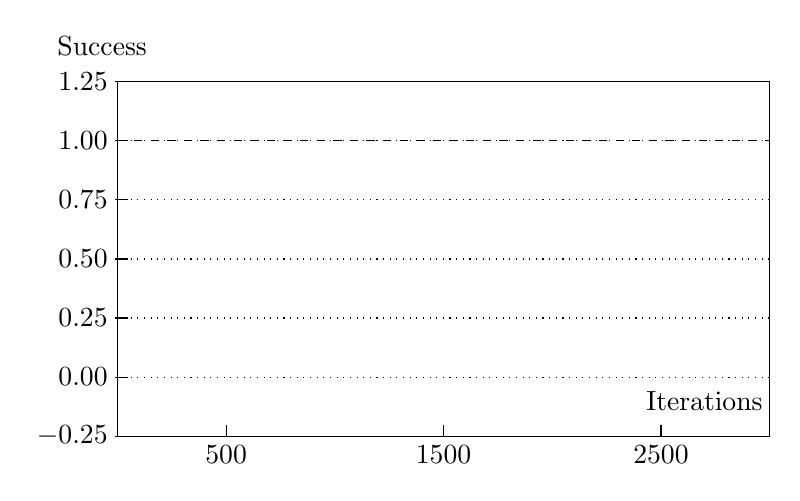
\begin{tikzpicture}[x=0.00276cm,y=3cm]
    % Draw the axes and grid lines
    \draw[-] (0,-0.25) -- (0,1.25) -- (3000,1.25) -- (3000,-0.25) -- cycle; 
    \draw[-,thin, dotted, ystep=0.25, xstep=3000] (0,-0.25) grid (3000,1.25);
    \foreach \x in {500, 1500, 2500}  \draw [-,xshift=0,yshift=-0.25](\x,-0.20) -- (\x,-0.25);
    \foreach \y in {-0.25,0.00,0.25,0.50,0.75,1.00,1.25}  \draw [-,yshift=0](4pt,\y) -- (-1pt,\y);
    \foreach \x/\xtext in {500/500, 1500/1500, 2500/2500} \node at (\x,-0.25) [below] {$\xtext$};
    \foreach \y/\ytext in {-0.25,0.00,0.25,0.50,0.75,1.00,1.25}  \node at (0,\y) [left] {$\ytext$};
    \node at (-70,1.4) {Success};
    \node at (2700,-0.1) {Iterations};
    \draw[-,red] plot[mark=x,mark size=4,mark options={color=red}] 
			file {figs/data/test05v3gmt.CP.tikzdata};
    \draw[-,blue] plot[mark=o,mark size=2,mark options={color=blue}] 
			file {figs/data/test05v3gmt.SP.tikzdata};
    % Also draw the expected convergence: 0.9^8 actions=0.43046
    \draw[dashed,-,yshift=0](0,1.0) -- (3000,1.0);

\end{tikzpicture}

   \caption{Performance of $\CLSELB$ (solid crosses) compared against $\CLSELA$ and $\BULSELA$ (both in dotted grey) in structure $\T_2$ using an applicability threshold of $0.2$.}
   \label{fig:performance-applicability}
\end{figure}


The above results show that the coverage-based confidence weighting can improve
the performance of the \CL\ approach in those cases where it performed poorly due
to false negative experiences, i.e., failure runs for a plan that includes
successful executions.
% %


Finally, we note that coverage-based selection weights encourage the agent to
explore all available options. This further ensures that all solutions are
systematically found, allowing the agent to decide which solution is optimal
faster. For some domains this may be an important feature.










%%%%%%%%%%%%%%%%%%%%%%%%%%%%%%%%%%%%%%%%%%%%%%%%%%%%
\section{Extended Framework: Event Types and Recursion}\label{sec:extended}
%%%%%%%%%%%%%%%%%%%%%%%%%%%%%%%%%%%%%%%%%%%%%%%%%%%%


\subsection{Event Types}



\subsection{Recursion}





%%%%%%%%%%%%%%%%%%%%%%%%%%%%%%%%%%%%%%%%%%%%%%%%%%%%
\section{Discussion and Conclusion}\label{sec:discussion}
%%%%%%%%%%%%%%%%%%%%%%%%%%%%%%%%%%%%%%%%%%%%%%%%%%%%

In this paper we propose a technique to enhance the typical plan selection
mechanism in BDI systems by allowing agents to learn and adapt the context
conditions of existing plans in the agent's plan library.
%%
As designing adequate context conditions that take full account of the agent's
environment for its complete life-cycle is often non-trivial, a framework that
allows for the \emph{refinement} of (initial) context conditions of plans
\textit{based on experience} is desirable. To this end we extend the BDI
framework to use \dt{}s as (part of) context conditions and provide a
probabilistic plan selection mechanism that caters for both exploration and
exploitation of plans.


We empirically evaluate two approaches to learning context conditions from experience, an aggressive approach that records and uses every outcome for learning, and a more conservative approach that records failure outcomes only when it considers the preceding choices that led to failure to be well-informed.
We confirm results from \cite{APSS08} that each approach has advantages in certain situations, but highlight an important shortcoming of the aggressive approach --- its complete inability to learn when applicability thresholds are used i.e. when the agent abandons plans with low chances of success. We then show that a new plan selection mechanism that also accounts for our confidence in the \dt\ classification can overcome the earlier issues with the aggressive approach. We conclude that the aggressive approach (that is also simpler), combined with the confidence measure (that also provides flexibility for tuning to different situations) is a better candidate for the general setting.

Our experiments do not consider the effects of conflicting interactions between sub-goals of a plan. For instance, if a sub-goal could succeed in more than one way causing different changes in the environment, one of which may in fact cause a subsequent sub-goal to fail, then in our current implementation it is not possible to detect and learn such interactions. Similarly we do not currently consider the effects of using failure recovery, under which alternative plans are tried upon the failure of a plan for achieving a goal. We note that both these features should be resolved for the real system. Moreover, we plan to do further experimentation with more realistic programs from existing applications. For continuous attributes, our approach requires that either the attributes be discretized or additional discrete attributes be used to test the continuous ones (for instance, check if temperature is $<20.5\textcelsius$).

One critique of the coverage-based confidence measure used is that it has a defined end state ($c_T(S)=1$) whereas for a real system, learning and re-learning will occur indefinitely as the agent continually tries to adapt to a changing environment. This implies that our confidence in a \dt's classification would also require calibration based on a changing environment. If the change in the environment was deliberate, then our confidence could be reset and subsequently \textit{re-built}. Without such an explicit signal the agent must rely on other methods for determining when the environment has changed significantly.

An appealing measure for recognising environmental changes is through the relatedness of its features. For instance, an observation that the grass is \textit{wet} presumably has a high correlation to the fact that it is \textit{raining}, and a \dt\ may (based on prior observations) very well use these factors in determining the likelihood of success of a plan to navigate the field. If then, we were to witness a world where it is not raining but the grass is wet (could be morning dew), then this world would be very different from the typical worlds we have seen so far and so we may have strong reason to reduce our confidence in the \dt\ classification of this new world.

The issue of combining learning and deliberative approaches for decision making in autonomous systems has not been widely addressed. In \cite{Riedmiller01} learning is used prior to deployment for acquiring low level robot soccer skills that are then treated as fixed methods in the deliberative decision making process once deployed. Hern\'andez et al. \cite{Hernandez04:Learning} give a preliminary account of how decision trees may be induced on plan failures in order to find an alternative logical context conditions in a deterministic paint-world example. More recently, in work related to BDI systems, \cite{Zhuo09:Learning} propose a method for learning hierarchical task network (HTN) method preconditions with partial observations in more complex domains. For this they first construct constraints from observed decomposition trees that are then solved offline using a constraint solver. In our work, learning and deliberation is integrated (as in \cite{APSS08}) such that one impacts the other and the classical exploration/exploitation dilemma applies. Initially, instead of following a random exploration policy (as is the case for agents with no initial knowledge), our agents are guided by the existing domain knowledge inherent in the BDI hierarchy.





%% The Appendices part is started with the command \appendix;
%% appendix sections are then done as normal sections
%% \appendix

%% \section{}
%% \label{}

%% References
%%
%% Following citation commands can be used in the body text:
%% Usage of \cite is as follows:
%%   \cite{key}         ==>>  [#]
%%   \cite[chap. 2]{key} ==>> [#, chap. 2]
%% 

%% References with bibTeX database:

\bibliographystyle{elsarticle-num}
\bibliography{hycas2010}

%% Authors are advised to submit their bibtex database files. They are
%% requested to list a bibtex style file in the manuscript if they do
%% not want to use elsarticle-num.bst.

%% References without bibTeX database:

% \begin{thebibliography}{00}

%% \bibitem must have the following form:
%%   \bibitem{key}...
%%

% \bibitem{}

% \end{thebibliography}


\end{document}

%%
%% End of file `elsarticle-template-num.tex'.
